\section{Μοριακά Νέφη και διαγαλαξιακός χώρος}
Στον μεσοαστρικό χώρο υπάρχει μια τεράστια ποσότητα ύλης υπό τη μορφή αερίου και σκόνης. Η ύλη αυτή, που μπορούμε να πούμε ότι είναι το πρωτόγεννες καύσιμο στη διαδικασία αστρικής δημιουργίας των γαλαξιών, αποτελείται περίπου κατά 99\% από αέριο και κατά 1\% από σκόνη με τη συνολική της μάζα για το δικό μας γαλαξία να είναι της τάξης των \SI{1e9}{ M_{\odot}}, ενώ η πυκνότητα της κυμαίνεται από \SIrange{1e-4}{1e6}{cm^{-3}}.

\begin{marginfigure}
	\label{fig:21}
	\centering
	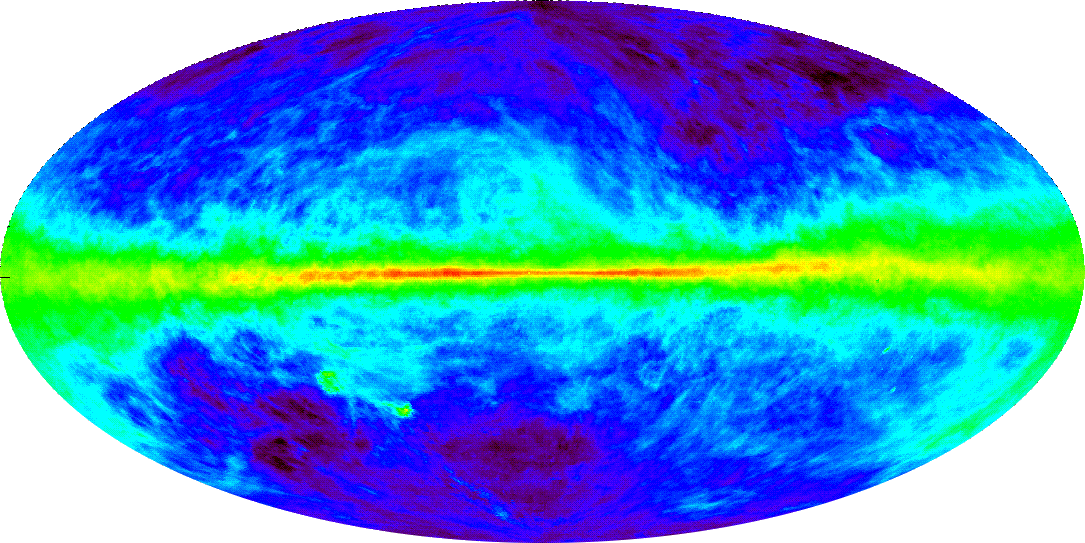
\includegraphics[width=1\linewidth]{Images/21.png}
	\caption{Εκπομπή του \ce{HI} στα 21.1 cm (Kalberla et al., 2005)%\cite{kalberla_2005}.
		H εκπομπή της γραμμής $21.1 \, cm$ στα ραδιοκύματα που οφείλεται στη μετάπτωση αντιστροφής του spin του πρωτονίου και του ηλεκτρονίου στη βασική κατάσταση του ατόμου του Υδρογόνου. Η ενεργειακή διαφορά των καταστάσεων είναι 
		$h \nu=\SI{6e-6}{eV}$, η οποία αντιστοιχεί σε μήκος κύματος \SI{21}{cm}.}
\end{marginfigure}

\begin{marginfigure}
	\label{fig:Ha}
	\centering
	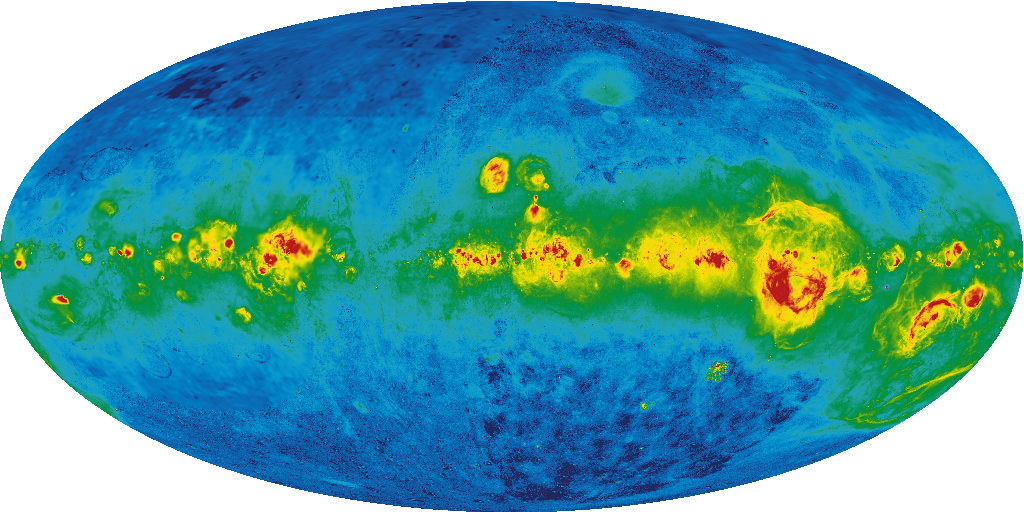
\includegraphics[width=1\linewidth]{Images/Ha.png}
	\caption{Εκπομπή Ha από συνδυασμό τριών διαφορετικών παρατηρήσεων (WHAM - VTSS - SHASSA) \cite{finkbeiner_2003}. Η εκπομπή Ha (\SI{656.28}{nm}) προέρχεται από την επανασύνδεση ιονισμένων ατόμων υδρογόνου κοντά σε θερμούς αστέρες O και B (\ce{HII} Regions).}
\end{marginfigure}


\paragraph{Μεσοαστρικό Αέριο} 
Το Μεσοαστρικό Αέριο παρατηρείται σε νεφελώδη μορφή και αποτελείται κυρίως (περίπου το 90\%) από υδρογόνο σε ατομική \ce{(H)}, ιονισμένη \ce{(HII)} και μοριακή \ce{(H2)} κατάσταση. Δεύτερο σε αναλογία είναι το Ήλιο \ce{(He)} (περίπου 9\%) ενώ το υπόλοιπο 1\% είναι βαρύτερα στοιχεία (\ce{C},\ce{O},\ce{Ne},\ce{Mg},\ce{Fe}, κ.α.) και μόρια (\ce{CO},\ce{CS}, κ.α.).


\paragraph{Μεσοαστρική Σκόνη}
%\begin{figure}[h]
%	\centering
%	\includegraphics[width=\medpage]{images/dust_emission_planck.png}
%	\caption{Εκπομπή της σκόνης του Γαλαξία μας όπως τη χαρτογράφησε το Planck.\cite{planck_2014}}
%\end{figure}

Η Μεσοαστρική Σκόνη αποτελείται κυρίως από άνθρακα και πυρίτιο σε ενώσεις με Υδρογόνο, Οξυγόνο, Μαγνήσιο και Σίδηρο ενώ το μέγεθος των κόκκων της σκόνης κυμαίνεται από \SI{0.01}{\micro\meter} έως \SI{1}{\micro\meter} ακολουθώντας μια κατανομή δύναμης όπου τα μικρότερα μεγέθη είναι πολυπληθέστερα από τα μεγαλύτερα. 
Η Μεσοαστρική Σκόνη παρατηρείται στις σπείρες του Γαλαξία μας (αλλά και σε άλλους γαλαξίες) με τη χαρακτηριστική μορφή τεράστιων σκοτεινών "δρόμων" λόγω της επισκότισης των όπισθεν αστέρων που προκύπτει από την απορρόφηση και σκέδαση του ορατού φωτός.


\section{Φάσεις και χαρακτηριστικά της Μεσοαστρικής Ύλης}
Η Μεσοαστρική Ύλη (ISM) απαντάται σε τρεις φάσεις με διαφορετικά φυσικά και χημικά χαρακτηριστικά: 
\footnote{Για τα χημικά χαρακτηριστικά αναφερόμαστε στή σύνθεση των μορίων και στην αναλογία των στοιχείων. Στα φυσικά χαρακτηριστικά αναφερόμαστε στη πυκνότητα και τη θερμοκρασία της Ύλης} 
τη \textbf{ψυχρή}, με θερμοκρασίες κάτω των \SI{100}{\kelvin},
 πυκνότητα \SIrange{30}{50}{cm^{-3}} και ποσοστό ιονισμού κάτω του 0.1\%, που αποτελείται από μοριακό και ατομικό αέριο Υδρογόνου και σκόνη, τη \textbf{θερμή}, με θερμοκρασίες της τάξης των \SIrange{1e3}{1e4}{K}, πυκνότητες \SI{0.3}{cm^{-3}}, που αποτελείται από ατομικό και ιονισμένο άεριο Υδρογόνο (ποσοστό ιονισμού 2-20\%) και την \textbf{υπέρθερμη} που οφείλεται σε κρουστικά κύματα εκρήξεων supernova και αστρικών ανέμων με θερμοκρασίες τάξης \SI{1e6}{K} και πυκνότητες μικρότερες των \SI{0.01}{cm^{-3}}.

\marginpar{
	\begin{table}[H]
		\caption{Χαρακτηριστικά \newline της μεσοαστρικής ύλης}
		\label{tab:ISM}
		\begin{tabular}{p{2.5cm} c  c  c }
			\toprule
			\multirow{2}{*}{Κατηγορία}  & Θερμοκρασία & Πυκνότητα   \\ 
			& \si{(K)} & \si{(cm^{-1})}  \\
			\midrule
			Μοριακά Νέφη & 10-50 & \num{>1e3} \\
			Ψυχρά Νέφη \ce{HI}  & \num{100} & \num{30} \\
			Θερμό \ce{HI}  & \num{1e3} & \num{0.1} \\
			Θερμό \ce{HII}  & \num{1e4} & \num{1e-2} \\
			Περιοχές \ce{HII} &  \num{1e4} & \num{>100} \\
			Υπέρθερμο Ιονισμένο αέριο &  \numrange{1e6}{1e7} & \num{1e-3} \\
			\bottomrule
		\end{tabular}
	\end{table}
}

\subsection{Ενεργειακή ισορροπία}
\label{par:EnergyBalance}
Η κινητική θερμοκρασία \footnote{Το ψυχρό μεσοαστρικό αέριο λόγω της γενικά χαμηλής του πυκνότητας δεν βρίσκεται σε θερμοδυναμική ισορροπία. Επομένως όταν μιλάμε για θερμοκρασία αναφερόμαστε στη κινητική του θερμοκρασία.\cite[p. 28]{spitzer_1998}} της Μεσοαστρικής Ύλης κυμαίνεται σε ένα εύρος τιμών 6 τάξεων μεγέθους όπως παρατηρούμε και από τον πίνακα~\ref{tab:ISM}. Για να περιγράψουμε και να μοντελοποιήσουμε την ενεργειακή ισορροπία στη Μεσοαστρική Ύλη και άρα να εξηγήσουμε και τις παρατηρούμενες θερμοκρασίες θα πρέπει να υπολογίσουμε τις διαδικασίες θέρμανσης και ψύξης. 
Ενώ η κύρια διαδικασία ψύξης είναι η εκπομπή ακτινοβολίας είτε μέσω αυθόρμητης αποδιέγερσης ή αποδιέγερσης λόγω κρούσης, για τη θέρμανση έχουμε μια πληθώρα διαδικασιών οι οποίες μπορούν να ταξινομηθούν σε 3 κατηγορίες:

\begin{itemize}
	\item θέρμανση από πεδία ακτινοβολίας: φωτοηλεκτρική απορρόφηση σε ουδέτερα στοιχεία, φωτοδιάσπαση στα μόρια, φωτοιονισμός.
	\item θέρμανση μέσω συγκρούσεων: από τυρβώδες ροές, κρουστικά κύματα καταλοίπων supernova και κοσμικής ακτινοβολίας.
	\item θερμική ανταλλαγή μεταξύ της σκόνης και νεφών αερίου, αλληλεπίδραση ιονισμένου αερίου με μαγνητικά πεδία, βαρυτική κατάρρευση. 
\end{itemize}

%\subsection{Παρατηρήσεις της Μεσοαστρικής Ύλης}
%Η παρατήρηση και μελέτη της Μεσοαστρικής Ύλης ποικίλει αναλόγως τη φάση στην οποία βρίσκεται.
%\subparagraph{Εκπομπή 21.1 cm}
%%\begin{figure}[h]
%%	\label{fig:21}
%%	\centering
%%	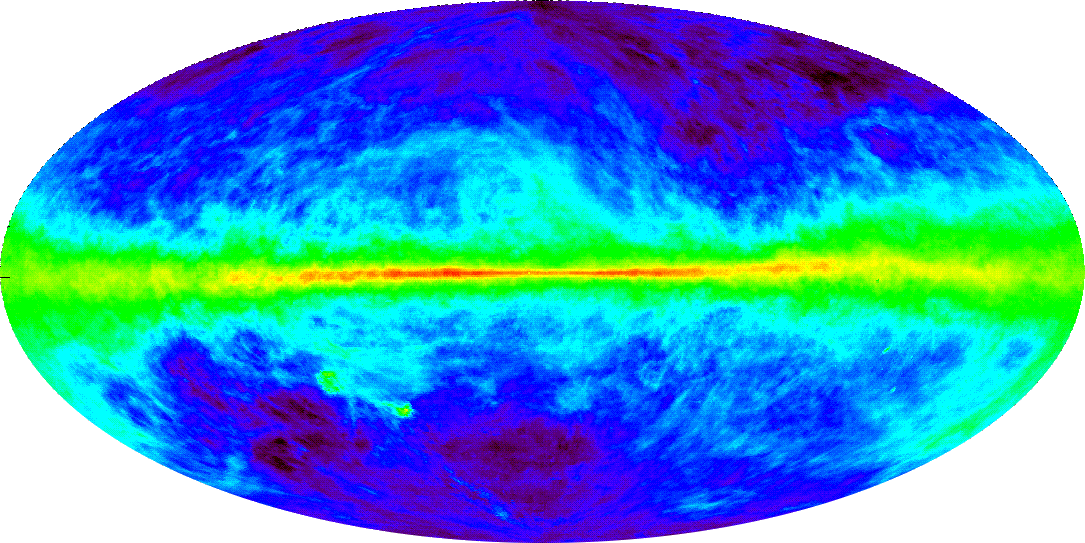
\includegraphics[width=\medpage]{images/21.png}
%%	\caption{Εκπομπή του \ce{HI} στα 21.1 cm (Kalberla et al., 2005)\cite{kalberla_2005}}
%%\end{figure}
%
%H καλύτερη μέχρι σήμερα δυνατή μέθοδος για την παρατήρηση του \textbf{Ουδέτερου Υδρογόνου \ce{H I}} είναι η εκπομπή της γραμμής $21.1 \, cm$ στα ραδιοκύματα που οφείλεται στη μετάπτωση αντιστροφής του spin του πρωτονίου και του ηλεκτρονίου στη βασική κατάσταση του ατόμου του Υδρογόνου. Η ενεργειακή διαφορά των καταστάσεων με συνολικό spin $F=1$ \textbf{(τα spin $p^+$ και $e^-$ είναι παράλληλα)} και $F=0$ \textbf{(τα spin $p^+$ και $e^-$ είναι άντιπαράλληλα)} είναι $h \nu=6\times 10^{-6} \, eV$, η οποία αντιστοιχεί στη γραμμή των 21 cm.
%Ο συντελεστής Einstein για την αυθόρμητη εκπομπή είναι $A_{10} \simeq 3\times 10^{-15}s^{-1}$ που αντιστοιχεί σε μια χρονική κλίμακα των $10^7$ ετών στην οποία παραμένει ένα διεγερμένο άτομο Υδρογόνου μέχρι να αποδιεγερθεί αυθόρμητα εκπέμποντας το παρατηρούμενο φωτόνιο. Ο πολύ μικρός αυτός ρυθμός εκπομπής αντιπαραβάλλεται εν τέλει από τη τεράστια ποσότητα του ατομικού υδρογόνου έτσι ώστε στατιστικά η γραμμή να είναι παρατηρήσιμη.
%
%\subparagraph{Εκπομπή \ce{H\alpha}}
%Κοντά σε αστέρες μεγάλης μάζας (φασματικού τύπου O και B) λόγω των φωτονίων υψηλής ενέργειας (μεγαλύτερες από το όριο Lyman) το αέριο υδρογόνο ιονίζεται. Οι περιοχές αυτές, ονομάζονται και Περιοχές HII, θα τις εξετάσουμε αναλυτικότερα στη παράγραφο~(\ref{par:HII regions}), και παρουσιάζουν έντονη εκπομπή ακτινοβολίας στη γραμμή Ha $(656.28\ nm)$ λόγω της επανασύνδεσης των ιονισμένων ατόμων.

%\begin{figure}[h]
%	\label{fig:Ha}
%	\centering
%	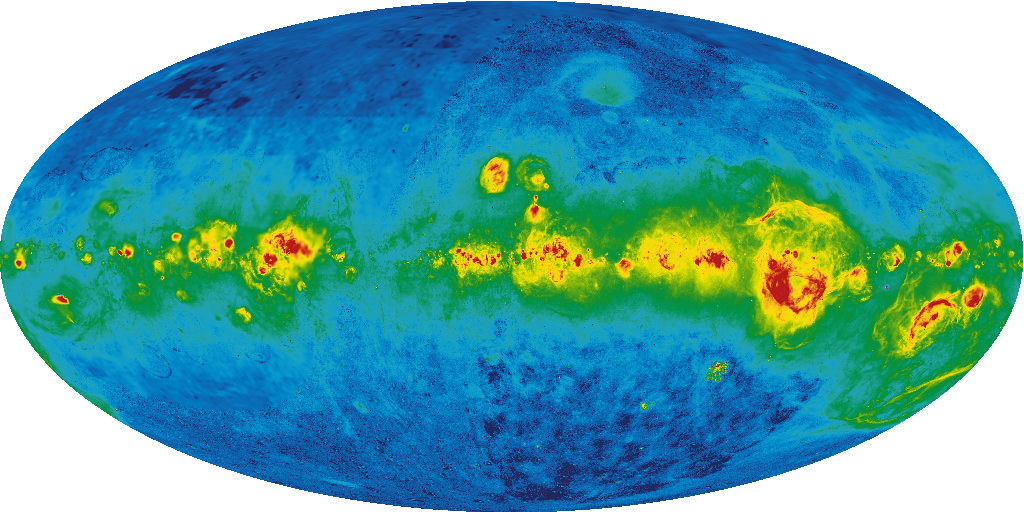
\includegraphics[width=\medpage]{images/Ha.png}
%	\caption{Εκπομπή Ha από συνδυασμό τριών διαφορετικών παρατηρήσεων (WHAM - VTSS - SHASSA) \cite{finkbeiner_2003}}
%\end{figure}
%

%===================================================================
%===================================================================
%===================================================================

\section{Μοριακά Νέφη}
%Οι πιο ενδιαφέρουσες, από τη σκοπιά της δημιουργίας αστέρων, περιοχές του Μεσοαστρικού Υλικού είναι τα Μοριακά Νέφη (Molecular Clouds).
Τα Μοριακά Νέφη είναι περιοχές όπου ψυχρή μεσοαστρική ύλη έχει πυκνότητες ικανοποιητικά μεγαλύτερες από τη μέση πυκνότητα του μεσοαστρικού υλικού έτσι η ιδιοβαρύτητα του νέφους να παίζει σημαντικό ρόλο στη δυναμική του. Καθώς το μοριακό νέφος καταρρέει, κατακρημνίζεται σε όλο και πιο συμπυκνωμένες δομές έως ότου η πυκνότητα και η μάζα σε μια τέτοια περιοχή είναι αρκετή ώστε να γεννηθούν νέοι αστέρες.   

\begin{marginfigure}
	\label{fig:CO}
	\centering
	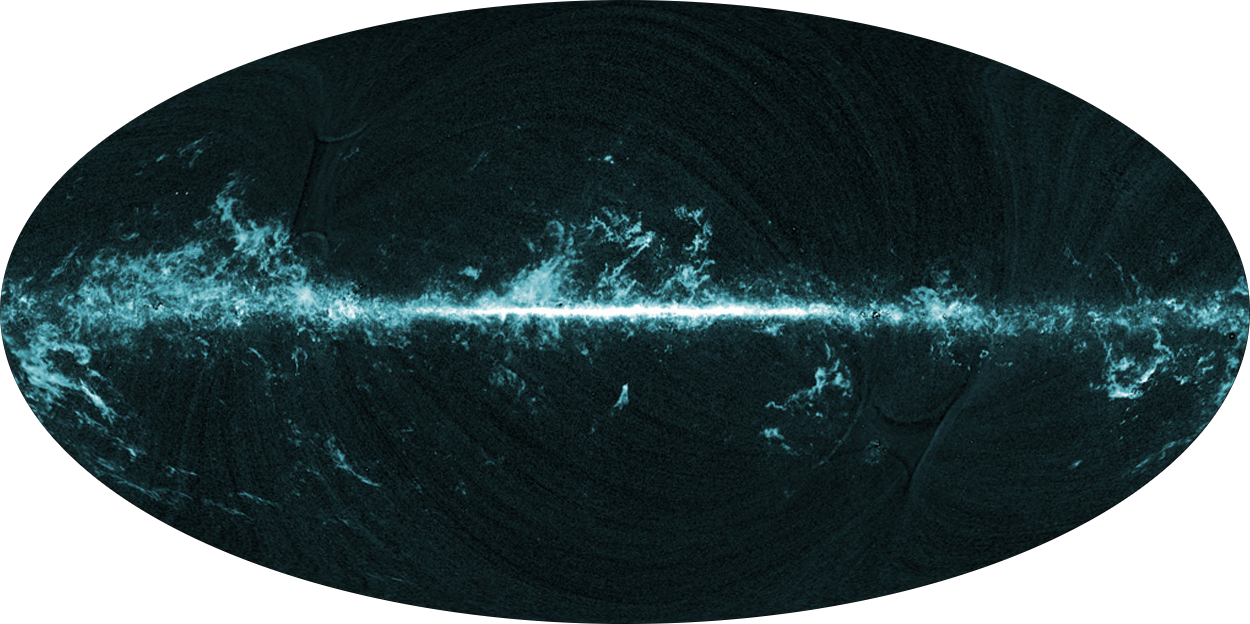
\includegraphics[width=1\linewidth]{Images/CO.png}
	\caption{Εκπομπή CO όπως τη χαρτογράφησε το Planck.\cite{planck_2014}.
		\newline
		Το \ce{H2} είναι ένα πλήρως συμμετρικό μόριο επομένως δεν έχει μόνιμη διπολική ροπή. Αυτό έχει σαν συνέπεια η διέγερση του να είναι σε θερμοκρασίες τις τάξεις των \SI{500}{K}. Άρα για τις τυπικές θερμοκρασίες των μοριακών νεφών $10-50\ K$ είναι αδύνατον να το παρατηρήσουμε άμεσα.
		\newline
		Ο εναλλακτικός τρόπος παρατήρησης του \ce{H2} είναι εμμέσως μέσω της εκπομπής διαφορετικών μορίων που είναι πιο "ευαίσθητα" στις χαμηλές θερμοκρασίες, όπως του \ce{CO} που είναι το δεύτερο σε αναλογία μόριο στο Σύμπαν και έχει μόνιμη διπολική ροπή (άρα έχουμε περιστροφικές ενεργειακές μεταβάσεις) πράγμα του επιτρέπει να εκπέμπει σημαντικά στο ραδιοφωνικό φάσμα.. 
		\newline
		H χαμηλότερη μετάβαση αντιστοιχεί σε θερμοκρασία \SI{5.5}{K} και αποδίδει ένα ραδιοφωνικό φωτόνιο στα \SI{2.6}{mm}.
	}
	%
	%Ο κύριος μηχανισμός διέγερσης ενός μορίου \ce{CO} στη $J=1$ είναι μέσω της σύγκρουσης του με ένα μόριο \ce{H2}. Αφού διεγερθεί η αποδιέγερση του μπορεί να γίνει είτε εκπέμποντας ένα φωτόνιο στα \SI{2.6}{mm} σε περιοχές με χαμηλή συνολική πυκνότητα είτε μεταφέροντας την ενέργεια του σε ξανά σε ένα μόριο \ce{H2} χωρίς να εκπεμφθεί φωτόνιο σε περιοχές με μεγάλη συνολική πυκνότητα.
	
\end{marginfigure}

Όπως φαίνεται και από το όνομα τους, τα Μοριακά Νέφη αποτελούνται κυρίως από μοριακό Υδρογόνο \ce{H2}. Στο γαλαξία μας πάνω από το 80\% του μοριακού Υδρογόνου βρίσκεται σε μοριακά νέφη κατανεμημένα πάνω στις σπείρες του δίσκου αλλά κυρίως σε ένα δακτύλιο ακτίνας 3 με 5 kpc από το κέντρο του γαλαξία \cite{rathborne_2009}.  Από παρατηρήσεις στο \ce{CO} τα μοριακά νέφη δείχνουν να έχουν μάζες που κυμαίνονται από \SIrange{1e3}{1e6}{M_\odot} με μια κατανομή νόμου δύναμης $-1.6$. \cite{stahlern_2004}

Για να δημιουργηθεί το Μοριακό Υδρογόνο καταλυτικό ρόλο παίζει η μεσοαστρική σκόνη.  Όταν δύο άτομα Υδρογόνου ενώνονται και δημιουργούν ένα μόριο \ce{H2} αυτό κερδίζει ενέργεια η οποία όμως δεν μπορεί να αποδοθεί στο περιβάλλον με αποτέλεσμα το μόριο να διασπάται. Παρολαυτά αν η διαδικασία αυτή γίνει πάνω σε έναν κόκκο σκόνης, τότε αυτός λειτουργεί καταλυτικά απορροφώντας το πλεόνασμα ενέργειας και το μόριο παραμένει σταθερό. Έτσι το ουδέτερο Υδρογόνο λειτουργεί σαν καύσιμο που τροφοδοτεί τις πυκνότερες περιοχές του μοριακού Υδρογόνου.

Ένα τυπικό μοριακό νέφος επιβιώνει για \SI{3e7}{yrs} πριν καταστραφεί από τους βίαιους αστρικούς ανέμους των αστέρων τύπου O και B που έχουν δημιουργηθεί στο εσωτερικό του. Κατά τη διάρκεια της ζωής του το νέφος αποδίδει τελικά ένα 3\% της μάζας του σε αστέρες. Έτσι για παράδειγμα αν θεωρήσουμε μια τιμή της συνολικής μάζας του μοριακού \ce{H2} στο Γαλαξιακό δίσκο \SI{2e9}{M_\odot} βρίσκουμε ότι ο ρυθμός δημιουργίας αστέρων (SFR) για το Γαλαξία μας είναι περίπου \SI{2}{M_\odot} ανά έτος.  

\subsection{Ενεργειακή ισορροπία στα Μοριακά Νέφη}
Όπως αναφέραμε γενικότερα στη παράγραφο~(\ref{par:EnergyBalance}) η θερμοκρασία ενός νέφους είναι αποτέλεσμα στης ενεργειακής ισορροπίας μεταξύ των μηχανισμών θέρμανσης και ψύξης. Για τα Μοριακά Νέφη συγκεκριμένα η θέρμανση είναι αποτέλεσμα της θερμότητας που παρέχεται από κοντινά άστρα ή μέσω της κοσμικής ακτινοβολίας, ενώ η ψύξη επιτυγχάνεται μέσω διαδικασιών απορρόφησης και κρούσης με τα σωματίδια της σκόνης ή του αερίου.
Η ενέργεια τελικά αποδίδεται μέσω της υπέρυθρης ακτινοβολίας η οποία οφείλεται στην απορρόφηση και την εκπομπή των φωτονίων από το περιβάλλοντα αέριο και σκόνη.


\begin{table}
	\caption{Χαρακτηριστικά και διαφορετικοί τύποι Μοριακών Νεφών}
	\label{tab:MCtypes}
	\begin{tabular}{l c c c c}
		\toprule
		\multirow{2}{*}{Κατηγορία} & Μέση ακτίνα &  Θερμοκρασία & Πυκνότητα \ce{H2} & Μάζα \\ 
		& \si{(pc)} & \si{(K)} & \si{(cm^{-3})} & \si{(M_\odot)} \\
		\midrule
		Γιγαντιαίο Μοριακό Νέφος & \num{20} & \num{15} & \num{100} & \num{1e5} \\
		Μοριακό Νέφος & $5$ & $10$ & $300$ & $10^4$\\
		clump & $2$ & $10$ & $10^3$ & $10^3$\\
		Πυρήνας Νέφους & $0.08$ & $10$ & $10^5$ & $10$\\
		\bottomrule
	\end{tabular}
\end{table}